% detailed  presentation of a model, including justifications for design decisions

Figure \ref{fig:MultilevelArchitecture} shows the overview of the multivel architecture designed to capture the two use cases described in the Process Challenge.

% Expliquer que le use case XSure ne nécessitait pas l'extension de metamodèle requise pour le usecase Acme Software Developement Process

\subsection{Base metamodel for the Process Challenge}

\begin{figure*}
 \centering
    % 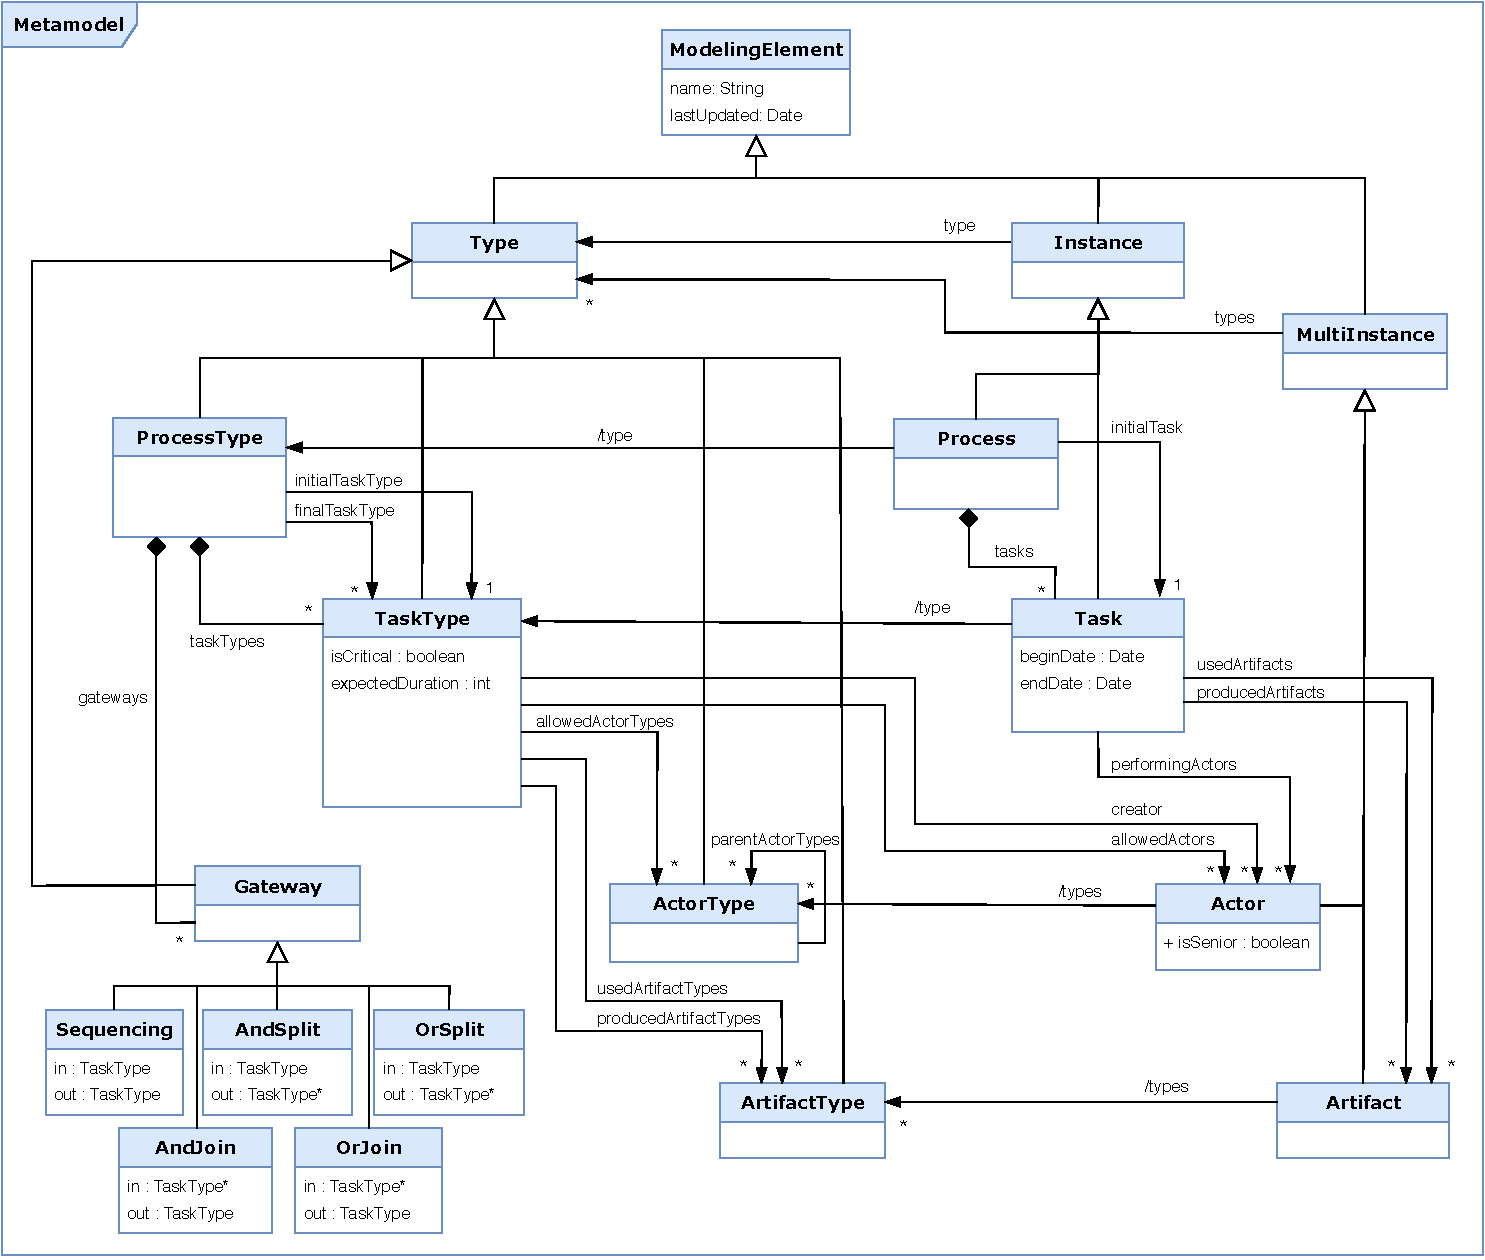
\includegraphics[width=1.0 \columnwidth]{Figures/Metamodel.pdf}
    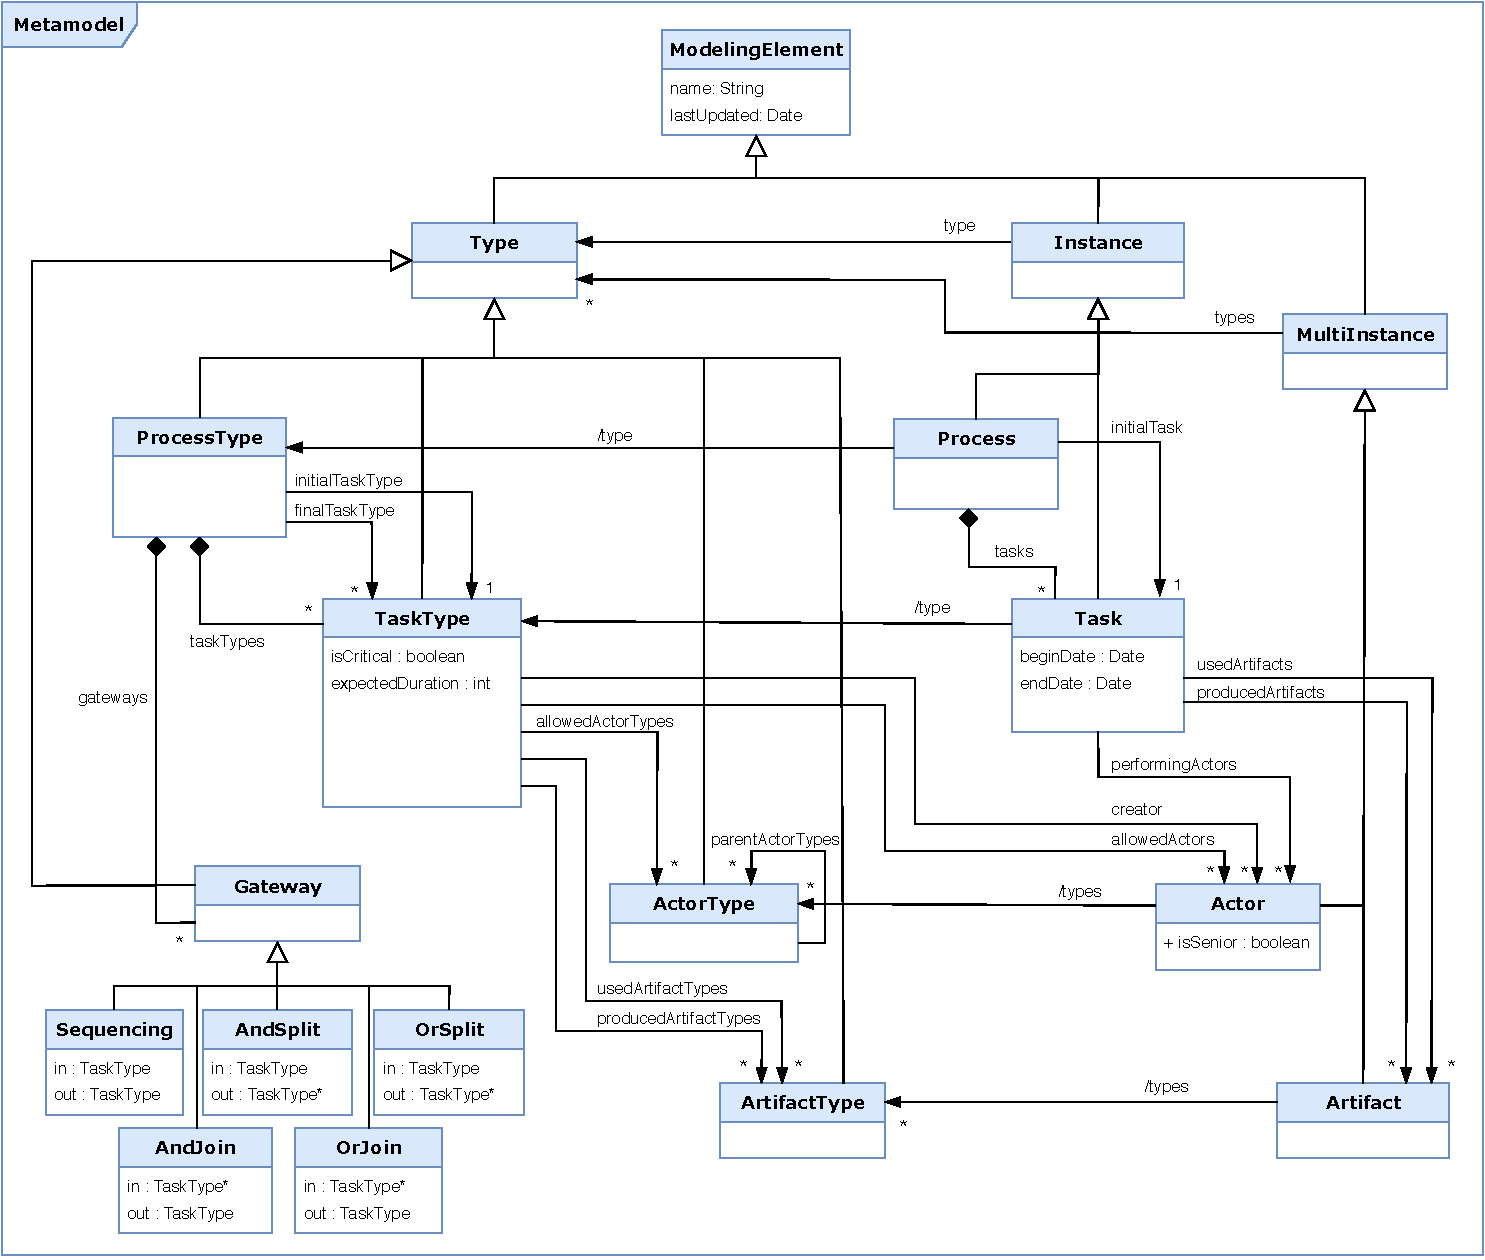
\includegraphics[width=1.0 \textwidth]{Figures/Metamodel.pdf}
     \caption{Process management base metamodel}
    \label{fig:BaseMetamodel}
\end{figure*}

\todo{Augmenter la taille des fontes}

In this section, we present and illustrate the base metamodel presented in figure \ref{fig:BaseMetamodel} with XSure insurance domain use case, whose a partial description was provided in the challenge description. Note that the capture of the requirements P1 to P19 in the context of XSure insurance domain are straightforward implementable while instantiating \textit{XSure model}, as an instance of base metamodel (the left side of figure \ref{fig:MultilevelArchitecture}).

Figure \ref{fig:BaseMetamodel} represents this base metamodel with a UML-like formalism, well adapted to represent object-oriented FML concepts and their instances. Our proposition relies on ontologic instantiation as presented in figure \ref{fig:LinguisticAndOntologicInstantiation}, with a common root concept \textit{ModelingElement}. Two types of ontological instantiation are needed to meet the requirements of the challenge. One provides that some instances conform to only one type (\textit{Process} and \textit{Task} do respectively conform to one \textit{ProcessType} and \textit{TaskType}) while some entities define their conformity to several types (\textit{Actor} and \textit{Artifact} do respectively conform to several \textit{ActorType} and \textit{ArtifactType}). This instantiation is reified with the relations \textit{type} and \textit{types} between \textit{Type}, \textit{Instance} and \textit{MultiInstance} concepts.  

% P1 : ProcessType / TaskType
% P2 : Gateways
% P3 : initial / final TaskTypes
% P4 : attribut creator dans TaskType > facile car même MM
% P5 : ActorType allowedActorTypes
% P6 : Actor allowedActors
% P7 : même chose pour ArtefactType avec used et produced
% P8 : attribut expectedDuration : TODO
% P9 : contrainte à mettre en place isCritical dans TaskType isSenior dans Actor : TODO
% P10: Process <> ProcessType
% P11: Tasks, toutes les TaskType sont instanciées en Task
% P12: begin et end date dans Task
% P13: instantiation des Artefacts et association des actors
% P14: 

\subsection{The Acme software development process}

\subsection{Openflexo tooling}

% Expliquer l'outillage construit et comment il marche


